\documentclass[12pt]{extarticle}
\usepackage[margin=1in]{geometry}
\usepackage{amsmath}
\usepackage{graphicx}

%My commands
\newcommand{\Prob}{\mathrm{Pr}}
\newcommand{\CDF}{\mathrm{CDF}}
\newcommand{\PDF}{\mathrm{PDF}}
\newcommand{\Exp}{\mathrm{E}}

\title{Monte Carlo Integration and the Metropolis Algorithm}
\author{Cody Petrie}

\begin{document}
\maketitle

\section{Background Information}

\subsection{Probability Theory}
Most of these next few sections are pulled from \cite{jarosz2008}. Here are some of the basics of probability theory. The cumulative distribution function (CDF) is the probability that a random variable ($X$) is less than or equal to some value ($x$).
\begin{equation}
  \CDF(x) = \Pr\{X \le x \}
  \label{equ:cdfdef}
\end{equation}
Note that this is always decreasing with the maximum value being 1. The derivative of this is then the probability distribution function (PDF), which describes the probability of $X$ being between $x$ and $dx$, where $dx$ is small.
\begin{equation}
  \PDF(x) = \frac{d}{dx} \CDF(x)
  \label{equ:pdfdef}
\end{equation}
Notice here that the PDF will always be positive because the CDF is monatonically increasing (always only increasing). Now using the definition of the PDF we can determine the probability that $X$ is between the values a and b by integrating,
\begin{equation}
  \Prob \{a \le X \le b\} = \int_a^b \PDF(x) dx.
\end{equation}

Now the expectation value, $\Exp[X]$, of is the value that is most likely to be chosen when choosing random values from $\PDF(X)$. Assuming $X$ is continuous it can be calculated by
\begin{equation}
  \Exp[X] = \int_{-\infty}^{\infty} x \PDF(x) dx.
\end{equation}
Obviously this integral goes to a sum if $X$ is discrete. Now if we define the random variable to be $Y=f(X)$ over the domain $[a,b]$, the expectation value of $Y$ becomes,
\begin{equation}
  \Exp[Y] = \int_a^b f(x) \PDF(x) dx.
  \label{equ:fullexp}
\end{equation}
The variance $\sigma^2[Y]$ is then given by
\begin{equation}
  \sigma^2[Y] = \Exp[(Y-\Exp[Y])^2].
  \label{equ:fullvar}
\end{equation}
Jarosz then goes on to list a few properties that can be found from the given information above. I will just list them here.
\begin{equation}
  \Exp[aY] = a \Exp[Y]
  \label{equ:constexp}
\end{equation}
\begin{equation}
  \sigma^2[aY] = a^2 \sigma^2[Y]
\end{equation}
\begin{equation}
  \Exp \left[ \sum_i Y_i \right] = \sum_i \Exp[Y_i]
  \label{equ:sumexp}
\end{equation}
\begin{equation}
  \sigma^2[Y] = \Exp[Y^2] - \Exp[Y]^2
  \label{equ:simpvar}
\end{equation}
\begin{equation}
  \sigma^2 \left[ \sum_i Y_i \right] = \sum_i \sigma^2[Y_i]
\end{equation}
Equation~\ref{equ:simpvar} shows up a lot in physics so I will take the time here to show it using the properties above. Start with equation~\ref{equ:fullvar} and expand to get
\begin{equation}
  \sigma^2[Y] = \Exp[Y^2 - 2Y\Exp[Y] + \Exp[Y]^2].
\end{equation}
Using equations~\ref{equ:constexp} and \ref{equ:sumexp} and noting the $\Exp[Y]$ is a constant we get
\begin{align}
  \sigma^2[Y] &= \Exp[ \Exp[Y^2] - 2Y\Exp[Y] + \Exp[Y]^2 ] \\
  &= \Exp[\Exp[Y^2]] - 2\Exp[Y]\Exp[Y] + \Exp[\Exp[Y]^2] \\
  &= \Exp[Y^2] - 2\Exp[Y]^2 + \Exp[Y]^2 \\
  &= \Exp[Y^2] - \Exp[Y]^2,
\end{align}
which is indeed the same as equation~\ref{equ:simpvar}.

%\subsection{The Mean-Value Theorem}

%\subsection{The Central Limit Theorem}

\section{Monte Carlo Integration}
Now I will apply what we have learned above to integrating a simple 1D function like $f(x)$ over the range $[a,b]$. I will not try to obtain an approximation for the integral
\begin{equation}
  I = \int_a^b f(x) dx.
\end{equation}
Start with the expectation value of $f(x)$.
\begin{align}
  \left< f(x) \right> &= \lim_{N \rightarrow \infty} \frac{1}{N} \sum_{i=1}^N f(X_i) \\
  &= \int_a^b f(x) \PDF(x) dx
\end{align}
Now if $X_i$ are pulled from a uniform distribution $U[a,b]$ then $\PDF(x)=1/(b-a)$ so we get
\begin{equation}
  I = \lim_{N->\infty} \frac{(b-a)}{N} \sum_{i=1}^N f(X_i).
\end{equation}
And thus we can approximate $I$ with
\begin{equation}
  I \approx \frac{(b-a)}{N} \sum_{i=1}^N f(X_i).
\end{equation}
This makes sence since it is like taking the average value of $f(x)$ and then multiplying it by the length of the integration interval.
This can be generalized to pulling $X_i$ from an arbitrary distribution by
\begin{equation}
  I \approx \frac{1}{N} \sum_{i=1}^N \frac{f(X_i)}{\PDF(X_i)}.
  \label{equ:mcint}
\end{equation}

Importance sampling is the technique of picking $\PDF(x)$ to be similar to $f(x)$ thus randomely choosing samples close to where $f(x)$ is ``important". It is probably important to mention here that the error goes as $N^{-1/2}$ regardless of dimension.
\subsection{Importance Sampling}
I will now go over the statement made in equation~\ref{equ:mcint} in more detail. If instead of pulling the samples $X_i$ from a uniform distribution (some of the $X_i$ may represent smaller parts of the integrand and be less important) it is wise to sample $X_i$ from a distribution that resembles the integrand. First let the integrand be $g(x) = f(x)/\PDF(x)$ where p(x) is the probability distribution that you want to sample from. Now the integral becomes
\begin{equation}
  I = \int_a^b f(x) dx = \int_a^b g(x) \PDF(x) dx.
\end{equation}
As before the last integral can be approximated as the average value of $g(x)$ and thus
\begin{equation}
  I \approx \frac{1}{N} \sum_{i=1}^\infty g(X_i) = \frac{1}{N} \sum_{i=1}^N \frac{f(X_i)}{\PDF(X_i)}.
\end{equation}

\section{The Metropolis Algorithm}
Much of this is pulled from \cite{kent1999} and \cite{foulkes2001}. Since we want $X_i$ to be pulled from a specific distribution $\PDF(x)$ it is often hard or impossible to do this by inverting $\PDF(x)$ and so we use the Metropolis algorithm. The Metropolis algorithm creates a random walk (sequence) of points that are distributed according to the distribution that you want.

The basic idea is that you start with a random number (or set of numbers, this is often called a walker in the literature) within the range that you need and then you generate another number (walker) that you propose to move to. If the random numbers are chosen from a uniform distribution then the probability of accepting the move is given by
\begin{equation}
  A(X' \rightarrow X) = \mathrm{min}\left( 1,\frac{\PDF(X')}{\PDF(X)} \right)
\end{equation}
If the move is not accepted then the next walker in the sequence is the same as the previous.

A simple Mathematica code showing an example of this for a Normal distribution is shown below. The resulting distribution is shown in figure~\ref{fig:exmetropolis}.
\begin{verbatim}
mu = 0; sig = 1;
P[x_] = 1/(sig*Sqrt[2 Pi])*Exp[-((x - mu)^2/(2*sig^2))];
num = 100000;
a = -5; b = 5;
dist = Table[0, {num}];
dist[[1]] = RandomReal[{a, b}];
For[i = 2, i <= num, i++, move = RandomReal[{a, b}];
 myrand = RandomReal[{0, 1}];
 If[P[move]/P[dist[[i - 1]]] >= myrand, dist[[i]] = move, 
  dist[[i]] = dist[[i - 1]];]]
A = 10000;
p1 = Histogram[dist];
p2 = Plot[A*P[x], {x, -10, 10}, PlotRange -> All, 
   PlotStyle -> {Thick, Red}];
Show[p1, p2]
\end{verbatim}

\begin{figure}
  \centering
  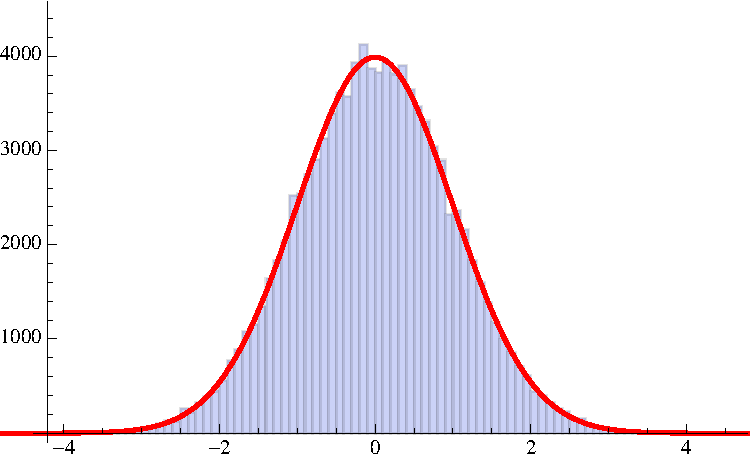
\includegraphics[width=0.5\textwidth]{exmetropolis}
  \caption{The histogram is of the random variables generated and the red curve is the original Normal distribution that I wanted to generate random variables from.}
  \label{fig:exmetropolis}
\end{figure}

\bibliographystyle{unsrt}
\bibliography{references}

\end{document}
